\subsubsection{WebRTC}

In 2011, the \glsreset{w3c}\gls{w3c} standardised the first version of \gls{webrtc} \cite{webrtc-w3c}. It was the first browser–native technology to enable \gls{p2p} connections for \gls{js} applications\footnote{To some extend, Adobe Flash and Java Applets already allowed \gls{p2p} connections, but required browser plugins primarily compatible with Desktop systems and are on their way to deprecation.}. Since then, adoption has spread to all major vendors \cite{webrtc-browser-compat} and its browser \glspl{api} have matured.

\gls{webrtc} is the only browser interface to the \gls{udp} transport layer. In contrast to the \gls{tcp}, which powers \gls{http} and \gls{ws} based communications, \gls{udp} is a so called "null protocol" \cite[p. 36]{high-performance-browser-networking}. This means, \gls{udp} does not take any measures to assure 1) packets arrive in order, 2) packets arrive at all, 3) connections preserve state or 4) the network does not congest. Consequently, \gls{udp} requires a lot less overhead than \gls{tcp} and performs better at time–sensitive applications like live media streaming.

\paragraph{Connection Negotiation}
Unlike web servers, web clients engaging in \gls{webrtc} connections are not publicly reachable by default. They are often connected to private networks and do not listen on ports on their network interface.
Hence a client needs to be informed of an inbound connection \textit{out–of–band}. With \gls{webrtc}, such connection intents are formalised by the \glsreset{sdp}\gls{sdp}. \gls{sdp} "is used to describe the 'session profile,' which represents a list of properties of the connection: types of media to be exchanged (audio, video, and application data), network transports, used codecs and their settings, bandwidth information, and other metadata" \cite[p. 323]{high-performance-browser-networking}.
The \gls{sdp} payload \cite[\S5]{sdp-rfc} can be exchanged through any application–specific channel. Many \gls{voip} systems use the \gls{sip}, while many public telephone networks use \gls{isup} \cite[p. 321]{high-performance-browser-networking}. Moreover channels like \gls{ws}, Bluetooth or even QR Codes could be used.

\begin{figure}
\centering
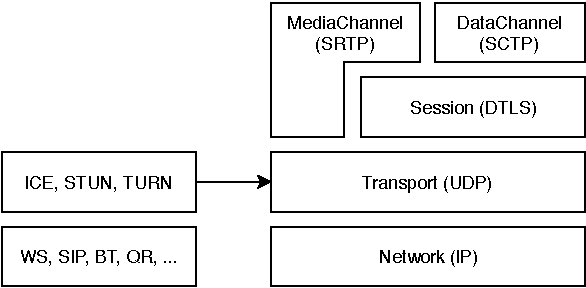
\includegraphics[width=0.75\textwidth]{graphics/webrtc-proto.pdf}
\caption{WebRTC stack, simplified from \citet[p. 316, fig. 18.3]{high-performance-browser-networking}}
\label{fig:webrtc-proto}
\end{figure}

\subsubsection{ICE Handshake}
What makes \gls{p2p} connection establishment so complex, is the broad employment of \gls{nat} devices. Most consumer and commercial networks as well as \glspl{mno} use \glspl{nat} to let clients inside a local network interface with the global internet.

Local devices establish connections to remote devices (like servers or peers) and the \gls{nat} maps their local \gls{ip} address and port tuple to a tuple consisting of the \gls{nat}'s \gls{ip} and a different port. If the \gls{nat} then receives a packet from the remote device on that port, it knows where to route it in the local network. This way, multiple devices can share a single \gls{ip} and are unreachable from the outside unless they initiated the connection. There are two basic categories of \glspl{nat} devices: symmetric and cone. The former will assign the external port randomly for any pair of local and remote device. This makes it impossible for a \gls{nat}ed device to determine its address using a stun server and pass it to a peer, because the peer will have a different \gls{ip} and the \gls{nat} will reject the connection. The latter type, cone \glspl{nat} can have restrictions on ports or remote addresses, but will generally assign a static port to local devices.

So, to establish a connection between two peers through a cone \gls{nat}, each peer would have to find out its public \gls{ip} address and the port its \gls{nat} exposes for it. The \glsreset{stun}\gls{stun} standardise how a devices can contact a dedicated public server and receive said public \gls{ip} and port. Optionally, the \gls{stun} request can be encrypted and be sent over \gls{udp} or \gls{tcp}.

However, in case of peers behind a symmetric \gls{nat}, the connection negotiation with an address reported by a \gls{stun} server would fail. To combat this issue, \gls{webrtc} applications can use \gls{turn} servers to relay connections to remote peers. This is a non–optimal solution, since it requires costly bandwidth and potentially defeats the purpose of \gls{p2p} solutions. In cases of user–generated content, like video–conferencing, it may nevertheless be the only option.

In a third scenario, the peers would share an \gls{ip} address space. The preferable routing would then be neither of the above, but a direct connection without \gls{nat} traversal.

\vref{fig:webrtc-handshake} shows an example of one peer behind a \gls{nat} and one publicly reachable peer establishing a connection through the \gls{ice} handshake.

There are many possible network constrains that can influence the \gls{webrtc} connection setup, like firewalls and \gls{vpn} configurations. The problem is, that client–side applications cannot know which network scenario is applicable to their current connection attempt and have to find out by trial and error. The process of gathering routing "candidates" and testing them in order of ascending complexity is referred to as \glsreset{ice}\gls{ice} \cite{ice-rfc}. Most modern browsers implement \gls{ice} – at least partially – in their \gls{webrtc} \gls{api} \cite{webrtc-browser-compat}. While \gls{ice} makes the connection process more reliable it can lead to significant wait times for users. A draft by \citet{trickle-ice} proposes a standard called \textit{Trickle} for aggregating candidates asynchronously on connection initiator and target, thus accelerating the connection establishment considerably.

\paragraph{Protocol Stack}
The \gls{webrtc} standard builds upon various proven protocols, that have already been in use by other telecommunication systems. Along dedicated media streaming, \gls{webrtc} also offers a data channel, that applications can use to exchange arbitrary messages. Media and data is sent over two different transmission protocols: \glsreset{srtp}\gls{srtp} and \glsreset{sctp}\gls{sctp} respectively. \vref{fig:webrtc-proto} visualises the stack of protocols in use. Both, \gls{srtp} and \gls{srtcp} packets, are transported via \gls{udp}. To overcome the lack of features (in comparison to \gls{tcp}), the \gls{webrtc} stack provides a set of tools: encryption can be achieved through \gls{dtls} and in-order delivery and transmission guarantees can be configured and are enforced in the application space, i.e. by the \gls{webrtc} browser implementation \cite[p. 319]{high-performance-browser-networking}.

\begin{figure}
\centering
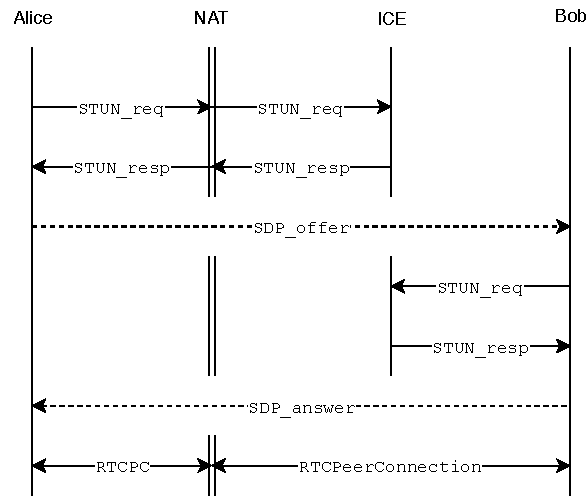
\includegraphics[width=0.75\textwidth]{graphics/webrtc-handshake.pdf}
\caption{WebRTC handshake example with Alice behind a \gls{nat} device and Bob with a public \gls{ip}. The dashed line represents \textit{out–of–band} communication.}
\label{fig:webrtc-handshake}
\end{figure}
